\documentclass[onecolumn, draftclsnofoot,10pt, compsoc]{IEEEtran}
\usepackage[utf8]{inputenc}
\usepackage{blindtext}
\usepackage[english]{babel}
%\usepackage{titlesec}
\usepackage{graphicx}
%\titlelabel{\thetitle.\quad}
%\titleformat{\section}{\bfseries\Large}{\thesection.}{0.5em}{}
%\titleformat{\subsubsection}{}{\thesubsubsection}{1em}{\itshape}
%\setcounter{secnumdepth}{4}

%\renewcommand\thesection{\arabic{section}}
%\renewcommand{\thesubsection}{\arabic{subsection}}
%\renewcommand{\thesubsubsection}{\arabic{subsubsection}}

\usepackage{setspace}
%\usepackage[style=numeric,sorting=nty]{biblatex}

%\addbibresource{mybib.bib}

%\title{Technology Review: Mixed Reality For Infrastructure Maintenance}
%\author{Team 20: Christopher C Cooper}
%\date{November 2018}

\usepackage{geometry}
\geometry{textheight=9.5in, textwidth=7in}

% 1. Fill in these details
\def \CapstoneTeamName{		xRLucid}
\def \CapstoneTeamNumber{		20}
\def \GroupMemberOne{			Christopher Cooper}
\def \GroupMemberTwo{			Austin Liang}
\def \GroupMemberThree{			David Okubo}
\def \GroupMemberFour{			Jonathan Chen}
\def \GroupMemberFive{			Mingyu Zhang}
\def \CapstoneProjectName{		Mixed Reality for Infrastructure Maintenance}
\def \CapstoneSponsorCompany{	OSU School of Civil and Construction Engineering}
\def \CapstoneSponsorPerson{		Yelda Turkan}

% 2. Uncomment the appropriate line below so that the document type works
\def \DocType{	%	Problem Statement
				Requirements Document
				%Technology Review
				%Design Document
				%Progress Report
				}

\newcommand{\NameSigPair}[1]{\par
\makebox[2.75in][r]{#1} \hfil 	\makebox[3.25in]{\makebox[2.25in]{\hrulefill} \hfill		\makebox[.75in]{\hrulefill}}
\par\vspace{-12pt} \textit{\tiny\noindent
\makebox[2.75in]{} \hfil		\makebox[3.25in]{\makebox[2.25in][r]{Signature} \hfill	\makebox[.75in][r]{Date}}}}
% 3. If the document is not to be signed, uncomment the RENEWcommand below
\renewcommand{\NameSigPair}[1]{#1}

%%%%%%%%%%%%%%%%%%%%%%%%%%%%%%%%%%%%%%%
\begin{document}
\begin{titlepage}
    \pagenumbering{gobble}
    \begin{singlespace}
    	\includegraphics[height=4cm]{coe_v_spot1}
        \hfill
        % 4. If you have a logo, use this includegraphics command to put it on the coversheet.
        %\includegraphics[height=4cm]{CompanyLogo}
        \par\vspace{.2in}
        \centering
        \scshape{
            \huge CS Capstone \DocType \par
            {\large November 30, 2018}\par
            \vspace{.5in}
            \textbf{\Huge\CapstoneProjectName}\par
            \vfill
            {\large Prepared for}\par
            \Huge \CapstoneSponsorCompany\par
            \vspace{5pt}
            {\Large\NameSigPair{\CapstoneSponsorPerson}\par}
            {\large Prepared by }\par
            Group\CapstoneTeamNumber\par
            % 5. comment out the line below this one if you do not wish to name your team
            \CapstoneTeamName\par
            \vspace{5pt}
            {\Large
                \NameSigPair{\GroupMemberOne}\par
                \NameSigPair{\GroupMemberTwo}\par
                \NameSigPair{\GroupMemberThree}\par
                \NameSigPair{\GroupMemberFour}\par
                \NameSigPair{\GroupMemberFive}\par
            }
            \vspace{20pt}
        }

%\begin{abstract}
%\end{abstract}
\end{singlespace}
\end{titlepage}
\newpage
\pagenumbering{arabic}
\tableofcontents
\listoffigures
%\listoftables
\clearpage

\textbf{Change History}\par

\begin{tabular}{ p{2cm} p{2cm} p{2cm} p{0.25\textwidth} p{0.25\textwidth} }
 \textbf{Revision} & \textbf{Date} & \textbf{Section} & \textbf{Original} & \textbf{New} \\
 \hline
 1.0 & 11/27/2018 & & & Creation of document first draft \\
  \hline
 1.1 & 03/31/2019 & Purpose & on a mobile tablet device. & on a mobile tablet device, specifically ones running android operating systems. \\
  \hline
 1.1 & 03/31/2019 & Scope & BIM & 3D \\
   \hline
 1.1 & 03/31/2019 & Scope & modify maintenance & modify and view maintenance \\
 \hline
 1.1 & 03/31/2019 & Scope &  & This maintenance information access will be implemented as a
stretch goal and is not part of requirements. \\
 \hline
 1.1 & 03/31/2019 & Product Overview & of the client but what the development team has decided to implement. & and will be implemented as a stretch goal. \\
  \hline
 1.1 & 03/31/2019 & Product Overview & BIM file will be downloaded and stored & obj file will be accessed from storage \\
  \hline
 1.1 & 03/31/2019 & Product Overview & from the BIM file & from the model file \\
  \hline
 1.1 & 03/31/2019 & External Interfaces & download, update, and upload BIM files. & download project files and upload maintenance issues. \\
  \hline
 1.1 & 03/31/2019 & Functions & Import/Load BIM from IFC files into the software. & Import/Load model from obj files into the software. \\
  \hline
 1.1 & 03/31/2019 & Functions & objects from the BIM file. & objects from the file. \\
  \hline
 1.1 & 03/31/2019 & Functions & The user can select a specific component of the 3D model to get more information on that object. & The user can select a files from the BIM360 project to get more information.
\end{tabular}

\clearpage

\section{Introduction}

    \subsection{Purpose}
    This document describes the functional and nonfunctional requirements of MR Maintain being created by xRLucid. MR Maintain will allow users to view BIM models in mixed reality on a mobile tablet device, specifically ones running android operating systems. Allowing them to view and modify BIM information, as well as a full-scale 3D model of the structure overlaying the physical structure in the real world.\par
    \subsection{Scope}
    MR Maintain is a mobile application that will allow users to access and see full 3D models overlaying the physical models in the real world. The application will additionally allow users to modify and view maintenance information associated with the structure through an intuitive MR interface. This maintenance information access will be implemented as a stretch goal and is not part of requirements.\par
        \subsection{Product Overview}
            \subsubsection{Product Perspective}
            \textit{User Interfaces}\par
            \hangindent=10mm\hangafter=0\noindent Mobile device will allow hardware and software keyboard input to edit information.\par
            \textit{Hardware Interfaces}\par
            \hangindent=10mm\hangafter=0\noindent No hardware interfaces are included.\par
            \textit{Software Interfaces}\par
            \noindent\hspace{10mm}Software Interface: Existing work flow of the client.\par
            \hangindent=15mm\hangafter=0\noindent MR Maintain will connect to the existing tool chain that the client uses to access and edit BIM data. This is not a requirement and will be implemented as a stretch goal.\par
            \noindent\hangafter=0\hspace{15mm}Upon transmission of edited data, software will notify users of the transmission's status.\par
            \textit{Communications Interfaces}\par
            \hangindent=10mm\hangafter=0\noindent No communication interface is included at this time.\par
            \textit{Memory}\par
            \hangindent=10mm\hangafter=0\noindent The obj file will be accessed from storage on the device for the software to display the 3D model. \par
            \textit{Operations}\par
            \hangindent=10mm\hangafter=0\noindent The device will utilized the camera to overlay objects from the model file to their real-life counterparts. The user will be able to select specific components to view a more detailed model as well as additional information. \par
            \textit{Site Adaptation Requirements}\par
            \hangindent=10mm\hangafter=0\noindent The devices GPS and camera's sensors will be used to pinpoint the user's location in relation to the object being examined. The camera will be used to keep objects anchored and overlaid onto the real-world components while the user moves around and interacts with the virtual objects. \par

            \subsubsection{Product Functions}
                   \hspace{10mm}FUNC 1: \hspace{10mm}Connect to cloud interface for BIM.\par
                   \hspace{10mm}FUNC 2: \hspace{10mm}Display 3D model from BIM overlaying real world structure.\par
                   \hspace{10mm}FUNC 3: \hspace{10mm}Access and edit BIM maintenance information.\par
                   \hspace{10mm}FUNC 4: \hspace{10mm}Submit edited BIM information to cloud.\par

            \subsubsection{User Characteristics}
               \hangindent=10mm\hangafter=0\noindent Maintenance Employee: The maintenance employee is the person/s that will be on site of a structure performing inspection/maintenance and logging inspection/maintenance data through MR Maintenance. They will also be viewing detailed BIM models over the real world structure. Training of employees may be needed.\par


            \subsubsection{Limitations}
            \hangindent=10mm\hangafter=0\noindent Limitations for the software include the use of mobile tablet device, restricting software to run on iOS and Android operating systems.\par
    \subsection{Definitions}
            \begin{table}[ht]
                \hspace{10mm}
                \begin{tabular}{l p{100mm}}
                   Building Information Model(BIM) & 3D model and data of a structure, recording all information from design to the structure's demolition [1].
                \end{tabular}
            \end{table}

\section{References}
    \hangindent=10mm\hangafter=0\noindent [1] Autodesk.com. (2018). What Is BIM. [Online] Available at: https://www.autodesk.com/solutions/bim [Accessed 29 Oct. 2018]. \par

\section{Specific Requirements}
    \subsection{External Interfaces}
        \hangindent=10mm\hangafter=0\noindent The software needs to be able to connect to the BIM 360 database to download project files and upload maintenance issues. The software itself can be used on any mobile device with a front-facing camera, accelerometer, gyroscope, GPS, and an internet connection. \par
    \subsection{Functions} % duplicate and tailor these sections for each of the functions listed in section 3.2 of this document
        %Define the fundamental actions that have to take place in the software in accepting and processing the inputs and in processing and generating the outputs, including
        \subsubsection*{a) Validity checks on the inputs}
            \hangindent=10mm\hangafter=0\noindent Using an on-screen keyboard in the software for input to prevent nonchar input errors. \par

        \subsubsection*{b) Exact sequence of operations}
        %\begin{itemize} %
            \hangindent=10mm\hangafter=0\noindent 1) Import/Load model from obj files into the software. \newline
            2) Render a 3D model of the objects from the file. \newline
            3) Pick anchor points in the real-world for the 3D model and match the virtual objects to the real-world structure based on the anchors. \newline
            4) Overlay the 3D model onto the real-world structure. \newline
            5) The software's 3D engine will keep the objects in position while the phone camera moves. \newline
            6) The user can select a files from the BIM360 project to get more information. \newline
            7) Access/edit maintenance info from BIM. \newline
            8) Save new updated maintenance info to the cloud database. \par
        %\end{itemize}
        \subsubsection*{c) Responses to abnormal situations}
            \hangindent=10mm\hangafter=0\noindent
            %1) Overflow \newline
            %2) Communication facilities \newline
            %3)
            Error handling and recovery \par
            \hangindent=15mm\hangafter=0\noindent
            Display an error message if: \par
            \hangindent=20mm\hangafter=0\noindent
                    - There is no backfacing camera on device. \newline
                    - There is no accelerometer, gyroscope, GPS. \newline
                    - No internet connection is available. \newline
                    - The software is given an unreadable BIM file. \newline
                    - Redo all checks if phone is locked then unlocked, relocate the device and re-anchor the objects. \newline
             \par
        \subsubsection*{d) Effect of parameters}
        Initial parameters of the software include the BIM model requested. This parameter impacts the 3D model to be rendered, as well as all information to be accessed from existing workflow.\par
         \subsubsection*{e) Relationship of outputs to inputs, including} %this is just a template right now, replace with actual text
        % \hangindent=10mm\hangafter=0\noindent
        %     1) Input/output sequences \newline
         %    2) Input of database address \newline
        %     3) Formulas for input to output conversion \newline
        %It may be appropriate to partition the functional requirements into subfunctions or subprocesses. This does not imply that the software design will also be partitioned that way. \par

        The relationship of output and input for this software will be mainly the user's satisfaction of how the BIM model requested is presented. The client and users satisfaction will be the output for the performance of software application implemented. The functions in the software will be considered as the input of this sequence.


    \subsection{Usability Requirements}
        Some important usability requirements that our team has established based off of H.C.I. usability specialists in our team are to make sure that all functions and options of functions are in a 'recall' from experience instead of having the user 'learn' how to operate and use our application. This means we will be incorporating the functions in a way that will have the user understand where the settings and functions like it is second nature to them. Another target our team established for usability requirements is to make sure our overall application is as simple to operate as possible, this means on the homepage of the application will ask the user whether or not they would like to use the tablet function or others options.

    \subsection{Performance Requirements}
       % Specify both the static and the dynamic numerical requirements placed on the software or on human interaction with the software as a whole. Static numerical requirements may include the following: \newline
       % \hangindent=10mm\hangafter=0\noindent
       %     a) The number of terminals to be supported; \newline
        %    b) The number of simultaneous users to be supported; \newline
        %    c) Amount and type of information to be handled. Static numerical requirements are sometimes identified under a separate section entitled Capacity.
       % \par
        %Dynamic numerical requirements may include, for example, the numbers of transactions and tasks and the amount of data to be processed within certain time periods for both normal and peak workload conditions. The performance requirements should be stated in measurable terms.
       % For example,
       %     95\% of the transactions shall be processed in less than 1 second.
       % rather than,
       %     An operator shall not have to wait for the transaction to complete.
       % NOTE Numerical limits applied to one specific function are normally specified as part of the processing subparagraph description of that function.
       \begin{itemize}
           \item A single user will be supported for use of the software.
           \item Software will access and handle one complete BIM model with relevant data.
           \item 90\% of all 3D models will be loaded and rendered in no more than twice the time for equivalent models to be loaded in Autodesk Revit.
           \item 90\% of all maintenance information transactions with the tool chain will be processed in less than 5 seconds(allowance made for mobile device in the field as expected platform).
       \end{itemize}

    \subsection{Logical Database Requirements}
        Information to be placed into a database will be placed utilizing the Autodesk Forge SDK. The SDK functions will manage inputs into the existing tools. Data entities and their properties are governed by these tools. Access to these entities will have a high frequency, estimated average of one access per minute of use.

    \subsection{Design Constraints}
         %Specify constraints on the system design imposed by external standards, regulatory requirements, or project limitations.

         Some design constraints that may occur is that there may be a limited way of using BIM and putting it into only using tablet devices. A personal error and issue our team has realized that we may face is the fact that if we build this application there would be some contract complications with IOS hardware, where as if we used tablets powered by androids it would be easier and less constricting when creating our application and using it.



    \subsection{Software System Attributes}
        %Specify the required attributes of the software product. The following is a partial list of examples:\newline
        \noindent a) Reliability% - Specify the factors required to establish the required reliability of the software system at time of delivery.\newline
        \begin{itemize}
            \item Utilize SDKs to ensure proper access to the existing work flow.
            \item Connect to existing work flow for proper storage of BIM data.
        \end{itemize}
        b) Availability% - Specify the factors required to guarantee a defined availability level for the entire system such as checkpoint, recovery, and restart.\newline
        \begin{itemize}
            \item Update existing work flow after each edit in case of need for recovery after error.
        \end{itemize}
        c) Security% - Specify the requirements to protect the software from accidental or malicious access, use modification, destruction, or disclosure. Specific requirements in this area could include the need to:
        %\begin{itemize}
         %   \item 1) Utilize certain cryptographic techniques
         %   \item 2) Keep specific log or history data sets
         %   \item 3) Assign certain functions to different modules
         %   \item 4) Restrict communications between some areas of the program
          %  \item 5) Check data integrity for critical variables
          %  \item 6) Assure data privacy
       % \end{itemize}
        \begin{itemize}
            \item Require login for access to tool chain.
            \item Assure privacy of login credentials.
        \end{itemize}

        \noindent d) Maintainability% - Specify attributes of software that relate to the ease of maintenance of the software itself.These may include requirements for certain modularity, interfaces, or complexity limitation. Requirements should not be placed here just because they are thought to be good design practices.\newline
        \begin{itemize}
            \item User Interface, user position tracking, and 3D model rendering should be kept modular to not only support maintenance of the software, but support upgrade potential to future MR devices.
        \end{itemize}
        e) Portability% - Specify attributes of software that relate to the ease of porting the software to other host machines and/or operating systems, including:
        %\begin{itemize}
        %    \item 1) Percentage of elements with host-dependent code;
        %    \item 2) Percentage of code that is host dependent;
        %    \item 3) Use of a proven portable language;
        %    \item 4) Use of a particular compiler or language subset;
        %    \item 5) Use of a particular operating system.
        %\end{itemize}
        \begin{itemize}
            \item 50\% of code, dependent on mobile device (i.e. phone, tablet) as hardware.
        \end{itemize}

    \subsection{Supporting Information}
    %The SRS should contain additional supporting information including
    %\begin{itemize}
    %   \item a) Sample input/output formats, descriptions of cost analysis studies, or results of user surveys;
    %    \item b) Supporting or background information that can help the readers of the SRS;
    %    \item c) A description of the problems to be solved by the software; d) Special packaging instructions for the code and the media to meet security, export, initial loading, or other requirements. The SRS should explicitly state whether or not these information items are to be considered part of the requirements.
    %\end{itemize}
    \begin{itemize}
        \item The problem to be solve is a lack of software to help maintenance employees visual maintenance information in the field with BIM models. This is to be considered part of the requirements.
        \item Software will be packaged using the Unity Game Engine to support all requirements of software deployment. This is not to be considered a part of the requirements.
    \end{itemize}

\newpage

\section{Verification}
    %Provide the verification approaches and methods planned to qualify the software. The information items for
   % verification are recommended to be given in a parallel manner with the information items in subclause 9.5.10 to 9.5.17.
    \subsection{External Interfaces}
        %indent later
        The software should be able to connect to the tool chain with whichever device it is installed on. There isn't one specific device that must be used, as long as the device meets the software's requirements.
    \subsection{Functions}
        An on-screen keyboard will be provided for user input to prevent input errors. When inspecting an object, the user will be able to import a BIM file from a model file after connecting to the tool chain. After loading the BIM file, the user sets anchor points in the real-world using the device's camera. These anchor points help overlay the real-world object with the virtual model from the BIM file. When the user physically moves, the virtual objects will continue to be an overlay on the real-world components. Selecting a specific component on the device will display more specific information for the user. The BIM can be modified using this software, and the file itself can be updated and uploaded into the cloud database.
        We will need to handle different situations when the software isn't functioning properly. When the app is first launched, it needs to check if the device has all of the necessary hardware and features needed to use the software properly. If the phone is ever locked while the app is in use, it will need to relocate the device and where it is located compared to the object being inspected. This ensures that the object overlay isn't corrupted by a lapse in connection.
        The function of this software is to be used to streamline maintenance inspections with construction. The user will be inputting different changes they want to make to objects being displayed on their device while seeing their changes updating the object, as well as the BIM file if they choose to update it.

    \subsection{Usability Requirements}
        The overall usability and function of the software should feel familiar for users who are experienced using other infrastructure software. The software should be simple enough for new users to operate with little to no experience.
    \subsection{Performance Requirements}
        The software will be able to load and use one BIM model including all of the information that comes with the model. Most 3D models will be able to be imported and processed on the mobile device at no more than double the time that Autodesk Revit will be able to load the same 3D models.
    \subsection{Logical Database Requirements}
    Database system is controlled by the existing workflow of the client. As such, there is no verification required for this software.
    \subsection{Design Constraints}
    No verification required for existing design constraints.
    \subsection{Software System Attributes}
    All tests involving the work flow integration will verify the existing tools, after inputs into the software, for updated values.
    \subsection{Supporting Information}
    Software will have acceptance testing by a select group of Civil Engineering students and instructors who are given a survey as to how they felt about the software being useful for on-site visualization of BIM information and if they would consider using it in the future. This test will aim for 80\% positive rating from surveys to verify that the software is useful for workers in the field.\par

\pagebreak
\section{Appendices}
\subsection{Assumptions and Dependencies}
    \begin{table}[ht]
        \begin{tabular}{l p{100mm}}
           Assumption 1: & Users have access to the existing tool chain with BIM models.
        \end{tabular}
    \end{table}
\subsection{Acronyms and Abbreviations}
    \begin{table}[ht]
        \begin{tabular}{l p{100mm}}
           MR & Mixed Reality\\
           BIM & Building Information Model
        \end{tabular}
    \end{table}

\pagebreak
\section{Gantt Chart}
    \begin{figure}[ht]
        \centering
            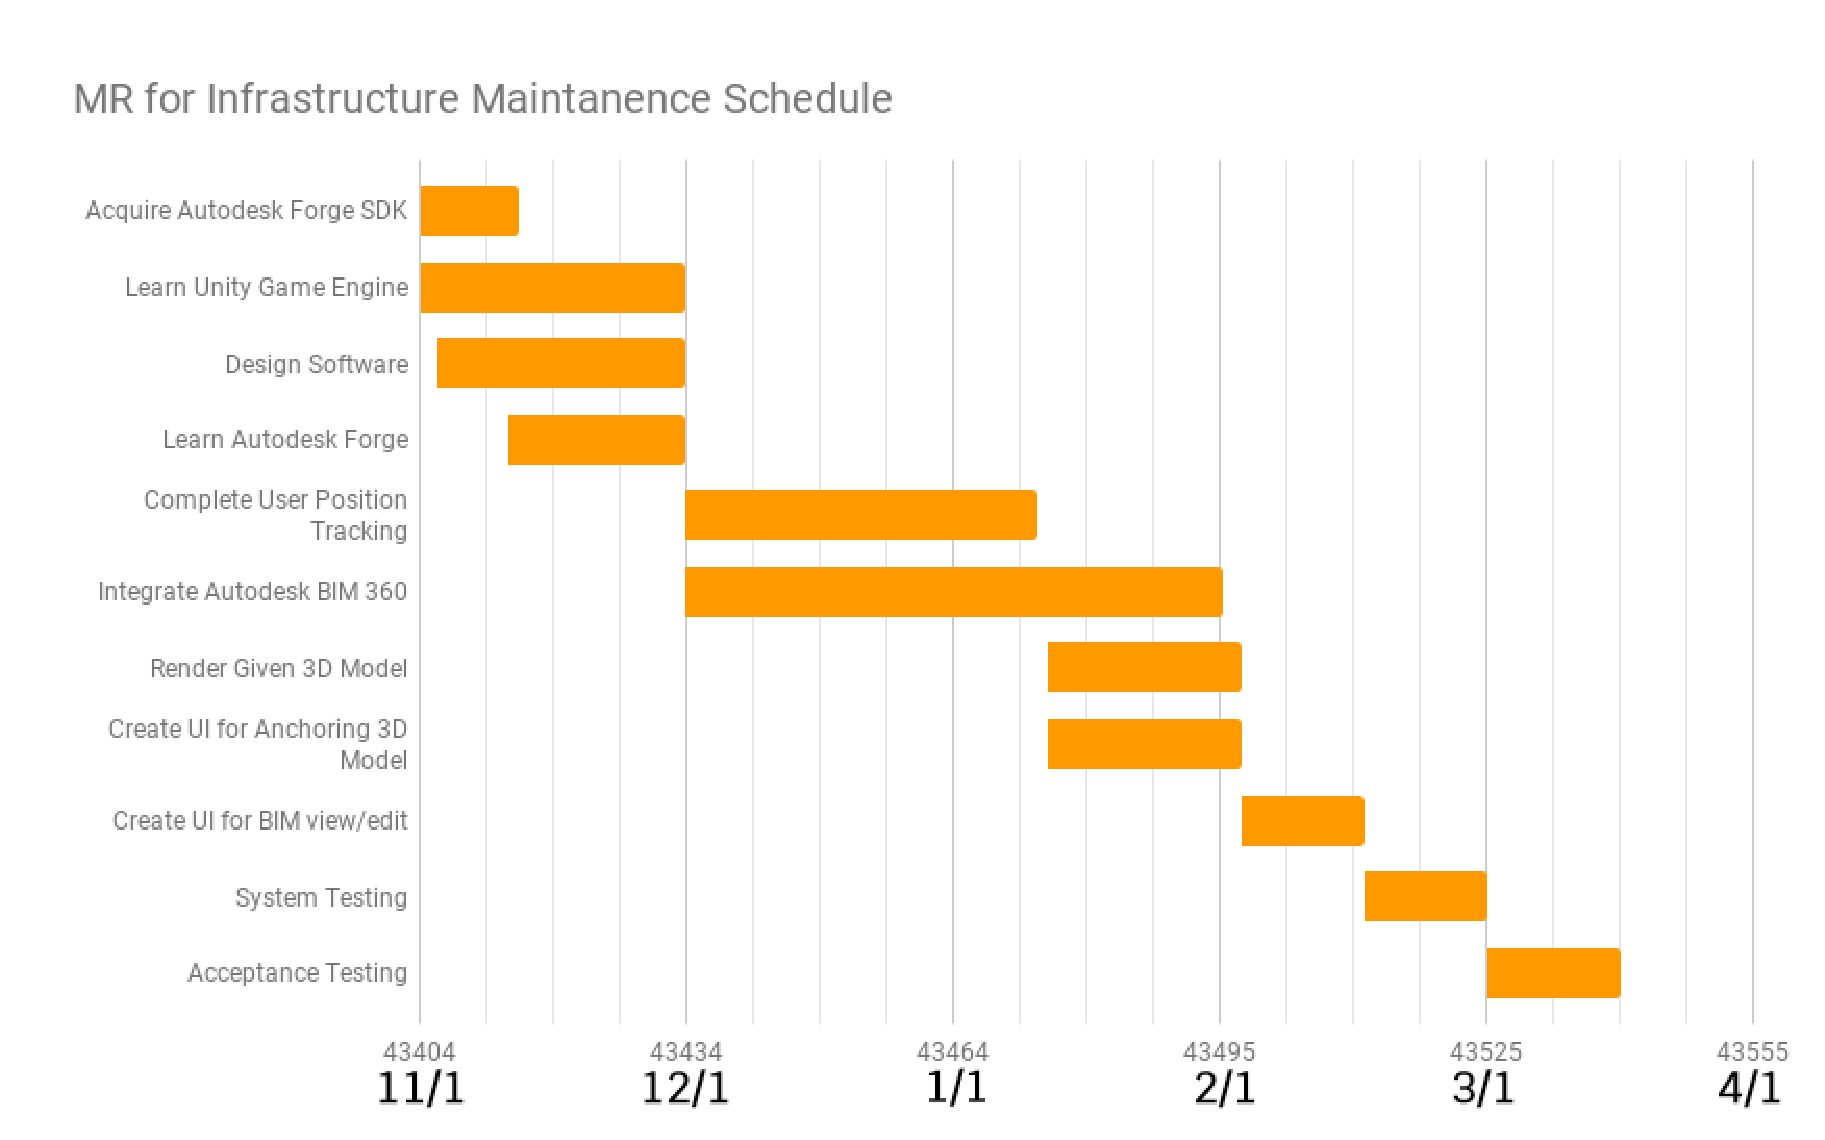
\includegraphics[width=1.0\textwidth]{schedule.eps}
        \caption{Tentative Schedule for Software Completion}
    \end{figure}

\end{document}
